\documentclass[a4paper,UTF8]{article}
\usepackage{amsmath}
\usepackage{amssymb}
\usepackage{amsthm}
\usepackage{bm}
\usepackage{color}
\usepackage{ctex}
\usepackage{enumerate}
\usepackage[margin=1.25in]{geometry}
\usepackage{graphicx}
\usepackage{hyperref}
\usepackage{tcolorbox}
\usepackage{algorithm}
\usepackage{algorithmic}
\theoremstyle{definition}
\newtheorem*{solution}{Solution}
\newtheorem*{prove}{Proof}
\newcommand{\indep}{\rotatebox[origin=c]{90}{$\models$}}
\usepackage{multirow}              
\usepackage{amssymb}% http://ctan.org/pkg/amssymb
\usepackage{pifont}% http://ctan.org/pkg/pifont
\setlength{\evensidemargin}{.25in}
\setlength{\textwidth}{6in}
\setlength{\topmargin}{-0.5in}
\setlength{\topmargin}{-0.5in}
% \setlength{\textheight}{9.5in}
%%%%%%%%%%%%%%%%%%此处用于设置页眉页脚%%%%%%%%%%%%%%%%%%
\usepackage{fancyhdr}                                
\usepackage{lastpage}                                           
\usepackage{layout}                                             
\footskip = 12pt 
\pagestyle{fancy}                    % 设置页眉                 
\lhead{2020年春季}                    
\chead{机器学习导论}                                                
% \rhead{第\thepage/\pageref{LastPage}页} 
\rhead{作业六}                                                                                               
\cfoot{\thepage}                                                
\renewcommand{\headrulewidth}{1pt}  			%页眉线宽,设为0可以去页眉线
\setlength{\skip\footins}{0.5cm}    			%脚注与正文的距离           
\renewcommand{\footrulewidth}{0pt}  			%页脚线宽,设为0可以去页脚线

\makeatletter 									%设置双线页眉                                        
\def\headrule{{\if@fancyplain\let\headrulewidth\plainheadrulewidth\fi%
		\hrule\@height 1.0pt \@width\headwidth\vskip1pt	%上面线为1pt粗  
		\hrule\@height 0.5pt\@width\headwidth  			%下面0.5pt粗            
		\vskip-2\headrulewidth\vskip-1pt}      			%两条线的距离1pt        
	\vspace{6mm}}     								%双线与下面正文之间的垂直间距              
\makeatother  


\begin{document}
	\title{机器学习导论\\
		习题六}
	\author{181220028, 李佩然, 181220028@smail.nju.edu.cn}
	\maketitle
	
	
	\section*{学术诚信}
	
	本课程非常重视学术诚信规范,助教老师和助教同学将不遗余力地维护作业中的学术诚信规范的建立。希望所有选课学生能够对此予以重视。\footnote{参考尹一通老师\href{http://tcs.nju.edu.cn/wiki/}{高级算法课程}中对学术诚信的说明。}
	
	\begin{tcolorbox}
		\begin{enumerate}
			\item[(1)] 允许同学之间的相互讨论,但是{\color{red}\textbf{署你名字的工作必须由你完成}},不允许直接照搬任何已有的材料,必须独立完成作业的书写过程;
			\item[(2)] 在完成作业过程中,对他人工作(出版物、互联网资料)中文本的直接照搬(包括原文的直接复制粘贴及语句的简单修改等)都将视为剽窃,剽窃者成绩将被取消。{\color{red}\textbf{对于完成作业中有关键作用的公开资料,应予以明显引用}};
			\item[(3)] 如果发现作业之间高度相似将被判定为互相抄袭行为,{\color{red}\textbf{抄袭和被抄袭双方的成绩都将被取消}}。因此请主动防止自己的作业被他人抄袭。
		\end{enumerate}
	\end{tcolorbox}
	
	\section*{作业提交注意事项}
	\begin{tcolorbox}
		\begin{enumerate}
			\item[(1)] 请在\LaTeX模板中{\color{red}\textbf{第一页填写个人的姓名、学号、邮箱信息}};
			\item[(2)] 本次作业需提交该pdf文件、问题3可直接运行的源码(BoostMain.py, RandomForestMain.py,不需要提交数据集),将以上三个文件压缩成zip文件后上传。zip文件格式为{\color{red}\textbf{学号.zip}},例如170000001.zip;pdf文件格式为{\color{red}\textbf{学号\_姓名.pdf}},例如170000001\_张三.pdf。
			\item[(3)] 未按照要求提交作业,或提交作业格式不正确,将会{\color{red}\textbf{被扣除部分作业分数}};
			\item[(4)] 本次作业提交截止时间为{\color{red}\textbf{6月11日23:59:59。本次作业不允许缓交,截止时间后不接收作业,本次作业记零分}}。
		\end{enumerate}
	\end{tcolorbox}
	
	\newpage




\section{\textbf{[25pts]} Bayesian Network}
贝叶斯网(Bayesian Network)是一种经典的概率图模型,请学习书本7.5节内容回答下面的问题:

(1) \textbf{[5pts]} 请画出下面的联合概率分布的分解式对应的贝叶斯网结构:
\begin{equation*}
\Pr(A, B, C, D, E, F, G) = \Pr(A)\Pr(B)\Pr(C)\Pr(D|A)\Pr(E|A)\Pr(F|B, D)\Pr(G|D, E)
\end{equation*}

(2) \textbf{[5pts]} 请写出图\ref{fig-DAG}中贝叶斯网结构的联合概率分布的分解表达式。
\begin{figure}[h]
\centering
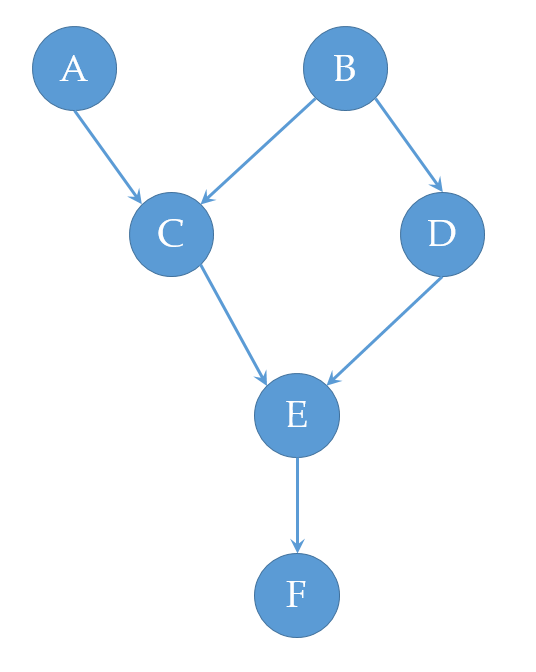
\includegraphics[scale=0.3]{bayes_net.png}
\caption{题目1-(2)有向图}
\label{fig-DAG}
\end{figure}
\newcommand{\cmark}{\ding{51}}%
\newcommand{\xmark}{\ding{55}}%

(3) \textbf{[15pts]} 基于第(2)问中的图\ref{fig-DAG}, 请判断表格\ref{table:DAG}中的论断是否正确。首先需要作出对应的道德图,并将下面的表格填完整。
\begin{table}[h]
\centering
\caption{判断表格中的论断是否正确}
\label{table:DAG}
\begin{tabular}{c|l|c||c|l|c}\hline
序号   		& 		关系  			& True/False 	& 序号   	& 		关系  			& True/False \\ \hline
1			&	$A \indep B$ 		& \cmark	    & 7  		& 	$F \perp B|C$ 		& \xmark	 \\
2			&	$A \perp B|C$ 	    & \xmark	    & 8  		& 	$F \perp B|C, D$ 	& \cmark	 \\
3			&	$C \indep D $		& \xmark	    & 9  		& 	$F \perp B|E$ 		& \cmark	 \\
4			&	$C \perp D|E$ 	    & \xmark	    & 10  		& 	$A \indep F $		& \xmark	 \\
5			&	$C \perp D|B, F$    & \xmark	    & 11  		& 	$A \perp F|C$ 		& \xmark	 \\
6			&	$F \indep B $		& \xmark	    & 12  		& 	$A \perp F|D$ 		& \xmark	 \\ \hline
\end{tabular}
\end{table}

\begin{solution}
\phantom{此处用于写解答(中英文均可)}

(1)见图\ref{fig-lpr}。
\begin{figure}[h]
\centering
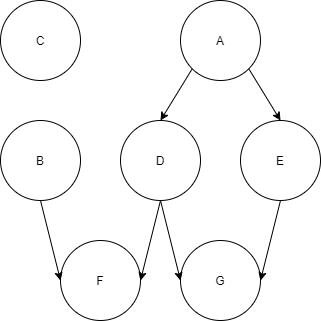
\includegraphics[scale=0.5]{Untitled2.png}
\caption{题目1-(1)有向图}
\label{fig-lpr}
\end{figure}

(2)图\ref{fig-DAG}中贝叶斯网结构的联合概率分布如下:
\begin{equation*}
\Pr(A,B,C,D,E,F) = \Pr(A)\Pr(B)\Pr(C|A,B)\Pr(D|B)\Pr(E|C,D)\Pr(F|E)
\end{equation*}

(3)首先做出第(2)问对应的道德图(见图\ref{fig-lpr1}):
表格将会直接填写在表\ref{table:DAG}中。
\begin{figure}[h]
\centering
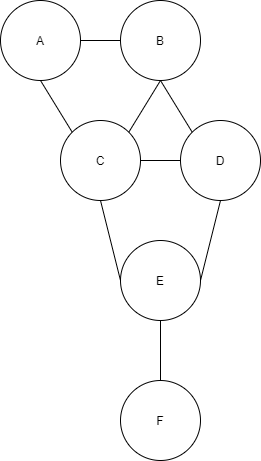
\includegraphics[scale=0.4]{Untitled.png}
\caption{题目1-(3)道德图}
\label{fig-lpr1}
\end{figure}
\end{solution}



\section{\textbf{[35$+$10pts]} Theoretical Analysis of $k$-means Algorithm}
给定样本集$\mathcal{D}=\left\{\mathbf{x}_{1}, \mathbf{x}_{2}, \ldots, \mathbf{x}_{n}\right\}$, $k$-means聚类算法希望获得簇划分$\mathcal{C}=\left\{C_{1}, C_{2}, \cdots, C_{k}\right\}$
使得最小化欧式距离
\begin{align} \label{eq1}
J\left(\gamma, \mu_{1}, \ldots, \mu_{k}\right)=\sum_{i=1}^{n} \sum_{j=1}^{k} \gamma_{i j}\left\|\mathbf{x}_{i}-\mu_{j}\right\|^{2}
\end{align}

其中$\mu_{1}, \ldots, \mu_{k}$为$k$个簇的中心(means), 
 $\gamma \in \mathbb{R}^{n \times k}$为指示矩阵(indicator matrix)定义如
下:若$\mathbf{x}_{i}$属于第j个簇, 则$\gamma_{i j}=1$, 否则为0,则最经典的$k$-means聚类算法流程如算法\ref{alg:alg1}中所示

{\begin{algorithm}[h]
		\caption{ $k-$means Algorithm }
		\label{alg:alg1}
		\begin{algorithmic}[1]{
				\STATE Initialize $\mu_{1}, \ldots, \mu_{k}$;
				\REPEAT
				\STATE {\bf{Step 1:}} Decide the class memberships of $\left\{\mathbf{x}_{i}\right\}_{i=1}^{n}$ by assigning each of them
				to its nearest cluster center.
				
				\begin{align}\gamma_{i j}=\left\{\begin{array}{ll}
				1, & \left\|\mathbf{x}_{i}-\mu_{j}\right\|^{2} \leq\left\|\mathbf{x}_{i}-\mu_{j^{\prime}}\right\|^{2}, \forall j^{\prime} \\
				0, & \text { otherwise }
				\end{array}\right.\end{align}
				\STATE {\bf{Step 2:}} For each $j \in\{1, \cdots, k\}$, recompute $\mu_j$ using the updated 
$\gamma$ to be	the center of mass of all points in $C_j$ :
			\begin{align}\mu_{j}=\frac{\sum_{i=1}^{n} \gamma_{i j} \mathbf{x}_{i}}{\sum_{i=1}^{n} \gamma_{i j}}
			\end{align}	
		
				\UNTIL the objective function J no longer changes;}
		\end{algorithmic}
		
\end{algorithm}}


(1) \textbf{[5pts]} 试证明, 在算法\ref{alg:alg1}中, Step 1和Step 2都会使目标函数J的值降低.

(2) \textbf{[5pts]} 试证明, 算法\ref{alg:alg1}会在有限步内停止。


(3) \textbf{[10pts]} 试证明, 目标函数J的最小值是关于$k$的非增函数, 其中$k$是聚类簇的数目。

(4) \textbf{[15pts]} 记$\hat{\mathbf{x}}$为$n$个样本的中心点, 定义如下变量,

\begin{table}[h]
	\centering
	\begin{tabular}{l}
		$T(X)=\sum_{i=1}^{n}\left\|\mathbf{x}_{i}-\hat{\mathbf{x}}\right\|^{2} / n$  \\
		$W_{j}(X)=\sum_{i=1}^{n} \gamma_{i j}\left\|\mathbf{x}_{i}-\mu_{j}\right\|^{2} / \sum_{i=1}^{n} \gamma_{i j}$  \\
		$B(X)=\sum_{j=1}^{k} \frac{\sum_{i=1}^{n} \gamma_{i j}}{n}\left\|\mu_{j}-\hat{\mathbf{x}}\right\|^{2}$  \\
	\end{tabular}
\end{table}

试探究以上三个变量之间有什么样的等式关系?基于此请证明, $k$-means聚类算法可以认为是在最小化$W_j(X)$的加权平均, 同时最大化$B(X)$.


(5) \textbf{[Bonus 10pts]}在公式\ref{eq1}中, 我们使用$\ell_{2^{-}}$范数来度量距离(即欧式距离), 下面我们考虑使用$\ell_{1^{-}}$范数来度量距离
\begin{equation}
\label{eq4}
J^{\prime}\left(\gamma, \mu_{1}, \ldots, \mu_{k}\right)=\sum_{i=1}^{n} \sum_{j=1}^{k} \gamma_{i j}\left\|\mathbf{x}_{i}-\mu_{j}\right\|_{1}
\end{equation}
\begin{itemize}
	\item 请仿效算法\ref{alg:alg1},给出新的算法(命名为$k-$means-$\ell_{1}$算法)以优化公式\ref{eq4}中的目标函数$J^{\prime}$. 
	\item 当样本集中存在少量异常点\href{https://en.wikipedia.org/wiki/Outlier}{(outliers)}时, 上述的$k-$means-$\ell_{2}$和$k-$means-$\ell_{1}$算法,	我们应该采用哪种算法?即哪个算法具有更好的鲁棒性?请说明理由。
\end{itemize}


\begin{solution}
	\phantom{此处用于写解答(中英文均可)}
	
(1) 对于\textbf{Setp 1},不妨设执行\textbf{Step 1}前的目标函数值为$\text{J}^\prime = \sum_{i=1}^{n} \sum_{j=1}^{k} \gamma^\prime_{i j}\left\|\mathbf{x}_{i}-\mu_{j}\right\|^{2}$,执行\textbf{Step 1}后的目标函数值为$\text{J} = \sum_{i=1}^{n} \sum_{j=1}^{k} \gamma_{i j}\left\|\mathbf{x}_{i}-\mu_{j}\right\|^{2}$。由\textbf{Step 1}的公式我们知道,对于给定的i,我们有$\sum_{j=1}^k \gamma_{ij}\left\|\mathbf{x}_{i}-\mu_{j}\right\|^{2}\leqslant \sum_{j=1}^k \gamma^\prime_{ij}\left\|\mathbf{x}_{i}-\mu_{j}\right\|^{2}$,因为当$\gamma_{ij}$在$j = 1, 2,\cdots,k$的时候只有一个值使为1,其余都为0,不妨设执行\textbf{Step 1}前这样的$\gamma_{ij}$为$\gamma_{ij_\star^\prime}$,执行\textbf{Step 1}后这样的$\gamma_{ij}$为$\gamma_{ij_\star}$,因而$\sum_{j=1}^k \gamma^\prime_{ij}\left\|\mathbf{x}_{i}-\mu_{j}\right\|^{2}=\left\|\mathbf{x}_{i}-\mu_{j_\star^\prime}\right\|^{2}$,$\sum_{j=1}^k \gamma_{ij}\left\|\mathbf{x}_{i}-\mu_{j}\right\|^{2}=\left\|\mathbf{x}_{i}-\mu_{j_\star}\right\|^{2}$,结合$\gamma_{ij_\star} = 1$的条件即可得到$\sum_{j=1}^k \gamma_{ij}\left\|\mathbf{x}_{i}-\mu_{j}\right\|^{2}\leqslant \sum_{j=1}^k \gamma^\prime_{ij}\left\|\mathbf{x}_{i}-\mu_{j}\right\|^{2}$。又因为对于每一个i都是如此,利用不等式的可加性,即可以得到J在\textbf{Step 1}里面是不增的。且在算法停止前一直单调减少,一旦不变算法即停止。

对于\textbf{Step 2},我们将J对$\mu_j,\quad j = \{1,2,\cdots,k\}$依次求偏导数,并令其为0,则可得到在此时若要让J取得最小值,$\mu_{j}=\frac{\sum_{i=1}^{n} \gamma_{i j} \mathbf{x}_{i}}{\sum_{i=1}^{n} \gamma_{i j}}$,所以第二问的做法可以让J取得当时的最小值,这是必然减少的,如果不减少也不会增加,此时算法停止。

(2) 当$\gamma$不变的时候,$\mu_i$在\textbf{Step 2}不会更新,这也就意味着此时此时的$J$将不变,算法中止,因而$\gamma$在算法执行时,每次都必须更新到一个之前从未出现过的状态上。设之前的状态为$S_1$,新的状态为$S_1^\prime=S_1$,
如果这两个状态相邻,则导致算法中止,否则则与(1)中的J在算法中递减互相矛盾。考虑到$\gamma$作为矩阵只有有限个元素,且每个元素只有有限个状态(0或1),因而$\gamma$也只有有限个状态可以被取得(不超过$2^{m\times k }$个状态),而算法的每次运行都会减少一种状态的出现,有限次后算法必然中止。

(3)首先,在k=1的条件下,那么它的最小值是$1,\cdots,\text{k}$中最小的。假设当$ \text{k}=\text{k}_0$时,它的最小值是$\text{k}=1,\cdots,\text{k}_0$中最小的,那么我们任意的加入一个新的簇$ C_{k+1}$,其簇中心为$\mu_{k+1}$,此时显然所有点都没有被分到该簇的,此时的J值与之前相同,而此时算法是可以继续进行下去的,这样子新的最小值一定小于旧的。综上,J的最小值是关于k的非增函数。

(4)首先,我们先给出给出等式:$$nB(X)+\sum_{i=1}^n\sum_{j=1}^n\gamma_{ij}W_j(X)=T(X)+K$$
下面,我们从左边开始化简:
\begin{align*}
\text{左边}&=\sum_{j=1}^{k} \sum_{i=1}^{n} \gamma_{i j}\left\|\mu_{j}-\hat{\mathbf{x}}\right\|^{2} +\sum_{j=1}^{k} \sum_{i=1}^{n}\gamma_{i j}(\sum_{i=1}^{n} \gamma_{i j}\left\|\mathbf{x}_{i}-\mu_{j}\right\|^{2} / \sum_{i=1}^{n} \gamma_{i j})\\
&=\sum_{j=1}^{k} \sum_{i=1}^{n} \gamma_{i j}(\left\|\mu_{j}-\hat{\mathbf{x}}\right\|^{2}+\left\|\mathbf{x}_i-\mu_j\right\|^{2})\\
&=\sum_{j=1}^{k} \sum_{i=1}^{n} \gamma_{i j}(\mathbf{x}_i^2+\hat{\mathbf{x}}^2+2\mu_j^2-2\hat{\mathbf{x}}\cdot\mu_j-2\hat{\mathbf{x}}\cdot\mu_j)\\
&=\sum_{j=1}^{k} \sum_{i=1}^{n} \gamma_{i j}(\mathbf{x}_i^2+\hat{\mathbf{x}}^2-2\mathbf{x}_i\cdot\hat{\mathbf{x}}+2\mathbf{x}_i\cdot\hat{\mathbf{x}}+2\mu_j^2-2\hat{\mathbf{x}}\cdot\mu_j-2\hat{\mathbf{x}}\cdot\mu_j)\\
&=\sum_{j=1}^{k} \sum_{i=1}^{n} \gamma_{i j}\left\|\mathbf{x}_{i}-\hat{\mathbf{x}}\right\|+K\\
&= \sum_{i=1}^{n}\left\|\mathbf{x}_{i}-\hat{\mathbf{x}}\right\|+K\\
&=nT(X)+K\\
&=\text{右边}
\end{align*}
下面证明, $k$-means聚类算法可以认为是在最小化$W_j(X)$的加权平均, 同时最大化$B(X)$。

由等式,我们可以直接发现$\sum_{i=1}^n\sum_{j=1}^n\gamma_{ij}W_j(X)=J$,所以最小化J就是在最小化$\sum_{i=1}^n\sum_{j=1}^n\gamma_{ij}W_j(X)$,而它即是$w_j(X)$的加权平均和。由于数据集是一个不变的数据集合,$\mathbf{x}_{i}$,$\hat{\mathbf{x}}$,$n$都是定值,所以$nT(X)$也是一个定值,所以当$w_j(X)$的加权平均和取得最小值的时候,$B(X)$也就取得了最大值。

(5)
\begin{itemize}
	\item  $k$-means-$\ell _1$聚类算法流程如算法\ref{alg:alg2}中所示

{\begin{algorithm}[h]
		\caption{ $k-$means-$\ell _1$ Algorithm }
		\label{alg:alg2}
		\begin{algorithmic}[1]{
				\STATE Initialize $\mu_{1}, \ldots, \mu_{k}$;
				\REPEAT
				\STATE {\bf{Step 1:}} Decide the class memberships of $\left\{\mathbf{x}_{i}\right\}_{i=1}^{n}$ by assigning each of them
				to its nearest cluster center.
				
				\begin{align}\gamma_{i j}=\left\{\begin{array}{ll}
				1, & \left\|\mathbf{x}_{i}-\mu_{j}\right\|_1 \leq\left\|\mathbf{x}_{i}-\mu_{j^{\prime}}\right\|_1, \forall j^{\prime} \\
				0, & \text { otherwise }
				\end{array}\right.\end{align}
				\STATE {\bf{Step 2:}} For each $j \in\{1, \cdots, k\}$, recompute $\mu_j$ using the updated 
$\gamma$ to be the median point of all points in $C_j$ :
			\begin{align}\mu_{j}=\text{median point of} \quad\{ x_{j}| r_{ij=1}\}
			\end{align}	
		
				\UNTIL the objective function $\text{J}^\prime$ no longer changes;}
		\end{algorithmic}
		
\end{algorithm}}

	\item $k$-means-$\ell_1$算法更合适。从统计的角度,使用中位数可以几乎无损失的排除异常点对于数据的影响,而使用平均数则会较为明显的反映在均值上。因此,$k$-means-$\ell _1$算法中使用中位点更有效。
\end{itemize}
\end{solution}


\section{[40pts] Coding: Ensemble Methods }

本次实验中我们将结合两种经典的集成学习思想:Boosting和Bagging,对集成学习方法进行实践。本次实验选取UCI数据集Adult,此数据集为一个二分类数据集,具体信息可参照\href{http://archive.ics.uci.edu/ml/datasets/Adult}{链接},为了方便大家使用数据集,已经提前对数据集稍作处理,并划分为训练集和测试集,数据集文件夹为adult\_dataset。

由于Adult是一个类别不平衡数据集,本次实验选用AUC作为评价分类器性能的评价指标,可调用\href{http://scikit-learn.org/stable/modules/generated/sklearn.metrics.roc_auc_score.html}{sklearn算法包}对AUC指标进行计算。

\begin{enumerate}[(1)]
	\item 本次实验要求使用Python3编写,要求代码分布于两个文件中,BoostMain.py, RandomForestMain.py ,调用这两个文件就能完成一次所实现分类器的训练和测试;
	
	\item \textbf{[35pts]} 本次实验要求编程实现如下功能:
	
	\begin{itemize}
		\item \textbf{[10pts]} 结合教材8.2节中图8.3所示的算法伪代码实现AdaBoost算法,基分类器选用决策树,基分类器可调用sklearn中\href{http://scikit-learn.org/stable/modules/generated/sklearn.tree.DecisionTreeClassifier.html}{决策树}的实现;
		\item \textbf{[10pts]} 结合教材8.3.2节所述,实现随机森林算法,基分类器仍可调用sklearn中决策树的实现,也可以手动实现,在实验报告中请给出随机森林的算法伪代码;
		\item \textbf{[10pts]} 结合AdaBoost和随机森林的实现,调查基学习器数量对分类器训练效果的影响 ,具体操作如下:分别对AdaBoost和随机森林,给定基分类器数目,在训练数据集上用5折交叉验证得到验证AUC评价。在实验报告中用折线图的形式报告实验结果,折线图横轴为基分类器数目,纵轴为AUC指标,图中有两条线分别对应AdaBoost和随机森林,基分类器数目选取范围请自行决定;
		\item \textbf{[5pts]} 根据参数调查结果,对AdaBoost和随机森林选取最好的基分类器数目,在训练数据集上进行训练,在实验报告中报告在测试集上的AUC指标;
	\end{itemize}
	
	\item \textbf{[5pts]} 在实验报告中,除了报告上述要求报告的内容外还需要展现实验过程,实验报告需要有层次和条理性,能让读者仅通过实验报告便能了解实验的目的,过程和结果。
	
\end{enumerate}

\noindent{\textbf{实验报告.}}

本次实验借助sklearn库的一部分工具,使用了Adaboost与RandomForest算法对数据集进行了预测,总体来说,当分类器数目较大时,RandomForest可以取得更优的效果,验证了课本的结论,此外,实验过程中也体会到了numpy包对科学计算的优化能力,在遇到第一版程序运行过慢的问题后,通过大量使用numpy库,运行速度得到了极大提升,可以进行较多轮迭代进行算法比较。

随机森林伪代码如下:

{\begin{algorithm}[h]
		\caption{ 随机森林伪代码 }
		\label{alg:alg2}
		\begin{algorithmic}[1]{
				\STATE 初始化迭代次数
				\REPEAT
				\STATE {\bf{Step 1:}} 随机挑选属性($\log_2(k)$个属性)
				\STATE {\bf{Step 2:}} 有放回随机挑选样本
				\STATE {\bf{Step 3:}} 训练模型、保存需要的属性、模型
		
				\UNTIL 达到迭代次数}
				\STATE {\bf{Step 4:}} 对于测试数据,依照保存模型对应的属性进行预测
				\STATE {\bf{Step 5:}} 对属性进行投票,得票最多(众数)即为随机森林模型的分类结果
		\end{algorithmic}
		
\end{algorithm}}


\begin{figure}[h]
\centering
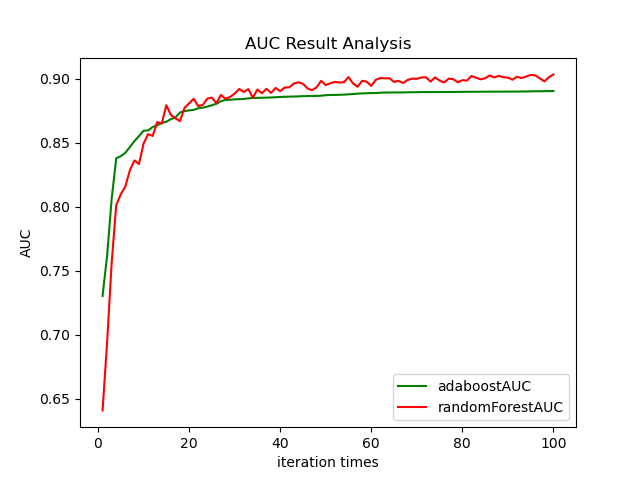
\includegraphics[scale=0.8]{Figure_1.png}
\caption{AUC对比图}
\label{fig-lprlpr}
\end{figure}

两种算法在训练集的AUC指标见图(\ref{123321}),训练共进行了100论,模型数目为1-100。两种算法选用最好的分类器数目,在测试集的AUC指标见表(\ref{tablelpr}):

总的来说,在测试集的表现与在训练集类似,表明数据集划分科学,样本均匀性较好,取得了不错的结果。

\begin{table} \label{tablelpr}
\caption{测试集算法AUC指标比较}  
\begin{center}  \label{123321}
\begin{tabular}{|l|l|l|l| p{5cm}|}  
\hline  
序号 & 算法&最优数目 & AUC  \\ \hline  
1 & Adaboost & 100 & 0.8917 \\ \hline  
2 & 随机森林 & 100 & 0.8957 \\ \hline
\end{tabular}  
\end{center}  
\end{table}

\end{document}